% CVPR 2027: replay buffer study. Single-file version.
% Needs cvpr.sty and ieeenat_fullname.bst from the author kit, plus cvpr-2027/papers.bib.
%
% Three overarching questions; the supervisor's seven questions are the sub-questions.
%   Q1  What does replay contribute when distillation is already present?
%         Q1   replay + distillation   : Intro (gist) -> Method (rationale, how) -> Results -> Discussion
%   Q2  How much should be stored, and which samples?
%         Q2a  budget                  : Intro (hypothesis) -> Results (true/false) -> Ablations
%         Q2b  image selection         : Method (pipeline) -> Results (summary) -> Ablations (detail)
%   Q3  In what form should samples be stored at a fixed memory budget?
%         Q3a  features vs. images     : Method (storage forms) -> Discussion -> Future directions
%         Q3b  same-memory features    : Discussion
%         Q3c  feature selection       : same as Q2b
%         Q3d  quantization            : Method (mention) -> Results (gist) -> Ablations + Discussion

\documentclass[10pt,twocolumn,letterpaper]{article}

%%%%%%%%% PAPER TYPE
% \usepackage{cvpr}              % CAMERA-READY version
\usepackage[review]{cvpr}      % REVIEW version
% \usepackage[pagenumbers]{cvpr} % arXiv version

% cvpr.sty already loads: xcolor, graphicx, amsmath, amssymb, booktabs,
% natbib, caption, subcaption, enumitem, cleveref
\usepackage{multirow}
\usepackage{xspace}

%%%%%%%%% Notes and macros
\newcommand{\TODO}[1]{\textbf{\color{red}[TODO: #1]}}
% \renewcommand{\TODO}[1]{}   % uncomment to hide TODOs
\newcommand{\Q}[1]{\textbf{Q#1}\xspace}     % research questions: \Q{1}, \Q{2}, \Q{3}
\newcommand{\Lce}{\mathcal{L}_{\text{CE}}}
\newcommand{\Lrep}{\mathcal{L}_{\text{rep}}}
\newcommand{\Lzscl}{\mathcal{L}_{\text{ZSCL}}}
\newcommand{\Lrd}{\mathcal{L}_{\text{RD}}}
\newcommand{\buf}{\mathcal{M}}      % replay buffer
\newcommand{\budget}{B}             % memory budget (bytes)

% Table helpers
\newcommand{\tbd}{\textcolor{gray}{--}}          % placeholder cell
\newcommand{\best}[1]{\textbf{#1}}
\newcommand{\pmstd}[1]{{\scriptsize$\pm$#1}}     % seed std, e.g. 86.17\pmstd{0.17}
\newcommand{\cmark}{\checkmark}
\newcommand{\xmark}{--}

\definecolor{cvprblue}{rgb}{0.21,0.49,0.74}
\usepackage[pagebackref,breaklinks,colorlinks,allcolors=cvprblue]{hyperref}

%%%%%%%%% PAPER ID
\def\paperID{*****}
\def\confName{CVPR}
\def\confYear{2027}

\title{\TODO{Title}: A Study of the Replay Buffer in Continual Learning of Vision-Language Models}

% Hidden in review mode
\author{First Author\\
Institution1\\
{\tt\small firstauthor@i1.org}
}

\begin{document}
\maketitle

%%%%%%%%%%%%%%%%%%%%%%%%%%%%%%%%%%%%%%%%%%%%%%%%%%%%%%%%%%%%%%%%%%%%%%%%%
\begin{abstract}
\TODO{Problem: replay is the default tool in CL, but the buffer itself is rarely studied.}
\TODO{What we study: what replay adds to distillation (\Q{1}); how much and which samples to store (\Q{2}); in what form to store them at a fixed memory budget (\Q{3}).}
\TODO{Setup: CLIP, MTIL, memory accounted in bytes.}
\TODO{Headline findings: one per question.}
\end{abstract}

%%%%%%%%%%%%%%%%%%%%%%%%%%%%%%%%%%%%%%%%%%%%%%%%%%%%%%%%%%%%%%%%%%%%%%%%%
\section{Introduction}
\label{sec:intro}

CLIP-style vision-language models have become the backbone for downstream image classification, but their zero-shot transfer capacity, built during large-scale pretraining, degrades rapidly once the model is adapted to new tasks. In the multi-task incremental learning (MTIL) setting~\cite{zheng2023zscl}, a model must process a sequence of classification tasks without revisiting earlier data, while retaining both per-task accuracy and pre-trained zero-shot capability. This creates a three-way tension: the model must be plastic (fitting each new task), stable (retaining previously trained tasks), and zero-shot preserving (maintaining pre-trained representations). These pressures map onto the Avg, Last, and Transfer metrics we report in \cref{sec:results}; existing methods typically improve one or two at the cost of the third.

% --- Q1: gist ---
\TODO{Gist of replay + distillation (\Q{1}): a small buffer of real exemplars combined with distillation toward the frozen pre-trained model is simple and competitive with methods that need a 900M-parameter generator. One or two sentences only; details in \cref{sec:method-rd}.}

% --- Gap ---
\TODO{Gap: the buffer is the main design knob, yet prior work treats it as a fixed hyperparameter and compares methods at a fixed number of samples, not bytes.}

% --- Q2a: hypothesis from known facts ---
\TODO{Hypothesis for \Q{2}: state it from known facts. \eg ``Because CLIP starts from a strong pre-trained representation and distillation already constrains the image encoder, we hypothesize that replay saturates at a small number of exemplars per class, so beyond this point what is stored matters more than how much.''}

We organize the study around three questions:
\begin{itemize}[leftmargin=*,itemsep=2pt]
  \item[\Q{1}] What does replay contribute when distillation is already present?
  \item[\Q{2}] How much should be stored, and which samples?
  \item[\Q{3}] In what form should samples be stored at a fixed memory budget?
\end{itemize}

\noindent\textbf{Contributions.}
\begin{itemize}
  \item \TODO{A byte-accounted benchmark protocol for replay in CLIP-based CL.}
  \item \TODO{A systematic study of \Q{1}--\Q{3}, with one finding per question.}
  \item \TODO{Practical recommendations.}
\end{itemize}

%%%%%%%%%%%%%%%%%%%%%%%%%%%%%%%%%%%%%%%%%%%%%%%%%%%%%%%%%%%%%%%%%%%%%%%%%
\section{Related Work}
\label{sec:related}

\paragraph{Vision-language models and zero-shot transfer.}
Contrastive Language-Image Pre-training (CLIP)~\cite{radford2021clip} aligns image-text pairs in a joint embedding space, yielding zero-shot transfer to unseen categories~\cite{lampert2009learning}. Fine-tuning CLIP distorts this geometry and degrades transfer~\cite{wortsman2022wiseft}, an effect compounded by sequential adaptation in the continual setting.

\paragraph{Regularization and replay.}
Catastrophic forgetting~\cite{mccloskey1989catastrophic} remains a central challenge in continual learning, where sequentially fine-tuned models tend to overwrite previously learned weights. Regularization-based methods address this by penalizing changes to parameters deemed important for past tasks: Elastic Weight Consolidation (EWC)~\cite{kirkpatrick2017ewc} approximates the posterior over weights via a Laplace approximation, anchoring critical parameters close to their previous values. Replay-based methods take a different route, rehearsing past data alongside new training. iCaRL~\cite{rebuffi2017icarl} maintains a bounded exemplar set and combines nearest-mean classification with knowledge distillation to preserve old class boundaries. DER++~\cite{buzzega2020der} extends this by storing soft logits alongside exemplars, adding a distillation term that stabilizes the model's output distribution across tasks. GDumb~\cite{prabhu2020gdumb} shows that a well-managed buffer alone is a strong baseline. These methods were designed for standard class-incremental settings and do not account for zero-shot transfer preservation.

\paragraph{Distillation for continual learning.}
Learning without Forgetting (LwF)~\cite{li2017lwf} introduced knowledge distillation as a mechanism for continual learning, using the model's predictions on new-task data as soft targets to constrain weight drift without requiring stored exemplars. However, this formulation is susceptible to the drifting reference problem: as the model is updated across tasks, the teacher signal is drawn from an evolving checkpoint whose predictions over out-of-distribution inputs become increasingly unreliable~\cite{li2017lwf}. ZSCL~\cite{zheng2023zscl} addresses this in the VLM setting by substituting the self-referential teacher with a fixed pre-trained CLIP backbone, whose predictions remain stable across the training sequence. This design sidesteps the drifting reference problem at the cost of requiring external image-text data to compute the anchor loss.

\paragraph{Parameter-efficient continual learning.}
Low-Rank Adaptation (LoRA)~\cite{hu2022lora} parameterizes weight updates as the product of two low-rank matrices inserted in parallel with frozen pre-trained weights. MoE-Adapters~\cite{yu2024moe} reduce cross-task interference via mixture-of-experts routing. ZAF~\cite{gao2024zaf} uses an EMA-updated LoRA adapter to stabilise zero-shot representations during sequential fine-tuning. C-CLIP~\cite{liu2025cclip} and SD-LoRA~\cite{wu2025sdlora} apply these ideas to continual CLIP adaptation. These methods share a common limitation: a single shared adapter must compress a growing sequence of tasks into a fixed parameter budget.

\paragraph{Generative replay for vision-language models.}
GIFT~\cite{gift2025} and LoRA-Loop~\cite{loraloop2025} represent the state of the art in synthetic replay for continual VLM learning. GIFT employs a frozen pre-trained diffusion model to regenerate both pretraining-distribution and downstream task data, applying contrastive distillation and adaptive weight consolidation over the generated image-text pairs. LoRA-Loop refines this by injecting task-specific LoRA adapters into the diffusion model itself. Both methods require a generative model (${\approx}900$M parameters) at training time, which is far larger than any replay buffer we study.

\paragraph{Exemplar selection.}
\TODO{Random, herding~\cite{welling2009herding,rebuffi2017icarl}, difficulty / surprisal (EL2N~\cite{paul2021el2n}), gradient coresets (GCR~\cite{tiwari2022gcr}), coverage ($k$-center~\cite{sener2018coreset}).}

\paragraph{Feature, latent, and compressed replay.}
\TODO{Latent replay~\cite{pellegrini2020latent}, REMIND~\cite{hayes2020remind} (product quantization~\cite{jegou2011pq} of mid-network features), feature adaptation for stale embeddings~\cite{iscen2020feature,yu2020sdc}, quantity vs.\ quality under data compression~\cite{wang2022compression}.}

%%%%%%%%%%%%%%%%%%%%%%%%%%%%%%%%%%%%%%%%%%%%%%%%%%%%%%%%%%%%%%%%%%%%%%%%%
\section{Method}
\label{sec:method}

\subsection{Problem setting and objective}
\label{sec:method-setting}
\TODO{MTIL: tasks $t=1,\dots,T$; buffer $\buf$ with byte budget $\budget$; CLIP image and text encoders; classification by cosine similarity to class-name text embeddings.}
\begin{equation}
  \mathcal{L} = \Lce + \lambda_{\text{rep}} \Lrep + \lambda_{\text{ZSCL}} \Lzscl + \lambda_{\text{RD}} \Lrd
  \label{eq:loss}
\end{equation}
\TODO{Define each term. $\Lce$: current task. $\Lrep$: CE on buffer samples against old class names. $\Lzscl$: distillation to frozen CLIP on reference data. $\Lrd$: same distillation on buffer images.}

\subsection{Replay + distillation (\Q{1})}
\label{sec:method-rd}
\TODO{Inspiration / rationale: ZSCL argued against replay; replay and distillation constrain different things (replay keeps old decision boundaries, distillation keeps zero-shot geometry). Gradient routing: $\Lzscl$ and $\Lrd$ compute teacher text embeddings without gradient, so they only constrain the image encoder; $\Lrep$ recomputes class-name embeddings with the live model and is the only term that updates the text encoder for previous classes.}
\TODO{How: batch composition, which teacher, which reference data.}

\subsection{Buffer construction pipeline (\Q{2}, \Q{3})}
\label{sec:method-pipeline}
\TODO{Data organization: when the buffer is filled (end of each task), how the budget is split across tasks and classes (equal per task vs.\ equal per class), and how samples are ranked within a class.}
\TODO{Selection strategies, with one line each: random; herding; surprisal maximization (define surprisal, \eg EL2N score or $-\log p(y\mid x)$ under the current model); GCR; coverage ($k$-center). The same strategies are applied in feature space for \Q{3}.}

\subsection{What is stored: images, embeddings, tokens (\Q{3})}
\label{sec:method-storage}
\TODO{Three storage forms. (i) Images (uint8). (ii) Final image embedding: replayed only through the text side, $\text{logits} = s \cdot \hat{z} \, G^\top$, where only the text embeddings $G$ carry gradient. (iii) Mid-network tokens (REMIND-style~\cite{hayes2020remind}): layers below the tap are frozen, so stored tokens cannot go stale.}
\TODO{Consequence: $\Lrd$ needs real pixels, so under feature storage it uses current-task images.}

\paragraph{Quantization (\Q{3}).}
\TODO{Embedding precision (fp32 / fp16 / int8 / int4) and product quantization~\cite{jegou2011pq} of tokens: $m$ sub-quantizers, codebook per task, bytes per sample. Codebook bytes count toward $\budget$.}

\subsection{Memory accounting}
\label{sec:method-memory}
All buffers are measured in bytes, not samples. \TODO{Define what counts toward $\budget$ (labels, codebooks, metadata).}
% Reference numbers (check against the pipeline):
%   raw image 224x224x3 uint8     = 150,528 B
%   ViT-B/16 embedding 512 fp32   =   2,048 B  (~73 per image)
%                       512 fp16  =   1,024 B  (~147 per image)
%                       512 int8  =     512 B  (~294 per image)
%   PQ tokens m=128               =  ~25.2 kB (~6 per image)
% NOTE: older logs report images as fp32 tensors (602 kB). Use uint8 everywhere.

%%%%%%%%%%%%%%%%%%%%%%%%%%%%%%%%%%%%%%%%%%%%%%%%%%%%%%%%%%%%%%%%%%%%%%%%%
\section{Experimental Setup}
\label{sec:setup}

\paragraph{Benchmark.}
We evaluate on the MTIL benchmark~\cite{zheng2023zscl}, which presents 11
classification datasets as a sequence of tasks: FGVC-Aircraft~\cite{maji2013fine}
(100 classes), Caltech-101~\cite{fei2004learning} (101),
CIFAR-100~\cite{krizhevsky2009learning} (100), DTD~\cite{cimpoi2014describing} (47),
EuroSAT~\cite{helber2019eurosat} (10), Flowers-102~\cite{nilsback2008automated} (102),
Food-101~\cite{bossard2014food} (101), MNIST~\cite{lecun1998gradient} (10),
Oxford-IIIT Pet~\cite{parkhi2012cats} (37), Stanford Cars~\cite{krause2013collecting}
(196), and SUN397~\cite{xiao2010sun} (397). Together they contain 1{,}201 classes
spanning fine-grained objects, textures, satellite imagery, digits, and scenes.
All study experiments use Order~I, the alphabetical order of~\cite{zheng2023zscl}
(Aircraft $\rightarrow$ Caltech-101 $\rightarrow \dots \rightarrow$ SUN397).
Order~II (Stanford Cars $\rightarrow$ Food $\rightarrow$ MNIST $\rightarrow$ Pet
$\rightarrow$ Flowers $\rightarrow$ SUN397 $\rightarrow$ Aircraft $\rightarrow$
Caltech-101 $\rightarrow$ DTD $\rightarrow$ EuroSAT $\rightarrow$ CIFAR-100) is used
only to check robustness to task order. ImageNet is never trained on. We
evaluate it after every task as a held-out measure of retained pre-training
knowledge. The backbone is CLIP ViT-B/16~\cite{radford2021clip}, and we fine-tune
all parameters of both the image and text encoders. Classification uses cosine
similarity between image embeddings and class-name prompt embeddings, with no
added classification head.

\paragraph{Metrics.}
Following~\cite{zheng2023zscl}, we report \textbf{Transfer}, \textbf{Avg.}, and
\textbf{Last}, computed from the accuracy matrix $a_{i,j}$, the accuracy on
task $j$ after training on task $i$, over the $T{=}11$ tasks.
\textbf{Transfer} measures how well zero-shot ability survives on tasks the
model has not been trained on yet. For each task $j>1$ we average
$a_{i,j}$ over the stages $i<j$ before task $j$ is learned, then average over
tasks (the upper triangle of the matrix, excluding the diagonal).
\textbf{Last} measures how much of each learned task is retained: the mean
accuracy over all tasks after the final stage, $\frac{1}{T}\sum_j a_{T,j}$.
\textbf{Avg.}\ is the mean of all $T\times T$ entries of the matrix. It covers
every task at every stage, so it reflects transfer, plasticity, and retention
together. ImageNet is never trained on and is excluded from all three
metrics.

\paragraph{Implementation details.}
\TODO{Optimizer, iterations per task, batch composition (current : replay ratio), seeds, compute.}

%%%%%%%%%%%%%%%%%%%%%%%%%%%%%%%%%%%%%%%%%%%%%%%%%%%%%%%%%%%%%%%%%%%%%%%%%
\section{Results}
\label{sec:results}

\subsection{Main results: replay + distillation (\Q{1})}
\label{sec:res-q1}
\TODO{Comparison with prior work (\cref{tab:sota}) and the component table (\cref{tab:q1}). Keep interpretation for \cref{sec:disc-q1}.}

\begin{table*}[t]
\centering
\small
\caption{\textbf{Comparison on MTIL} (CLIP ViT-B/16, 11 tasks). Transfer is
the upper-triangle mean (ZSCL convention). Extra memory is the replay
buffer or generator kept at training time.}
\label{tab:sota}
\begin{tabular}{@{}l l l r ccc@{}}
\toprule
Method & Venue & Replay & Extra memory & Transfer & Avg. & Last \\
\midrule
ZSCL~\cite{zheng2023zscl}       & ICCV'23  & reference data    & \tbd & \tbd & \tbd & \tbd \\
MoE-Adapters~\cite{yu2024moe}   & CVPR'24  & --                & \tbd & \tbd & \tbd & \tbd \\
GIFT~\cite{gift2025}            & CVPR'25  & synthetic (diff.) & \tbd & \tbd & \tbd & \tbd \\
LoRA-Loop~\cite{loraloop2025}   & ICCVW'25 & synthetic (diff.) & \tbd & \tbd & \tbd & \tbd \\
\midrule
% verify all prior-work numbers against the papers (upper-triangle Transfer)
Ours: image replay              & --       & images            & 1656\,MB & 68.79\pmstd{0.16} & 77.18\pmstd{0.01} & 86.28\pmstd{0.10} \\
Ours: best equal-memory         & --       & \tbd              & \tbd & \tbd & \tbd & \tbd \\
\bottomrule
\end{tabular}
\end{table*}

\begin{table}[t]
\centering
\small
\setlength{\tabcolsep}{4pt}
\caption{\textbf{\Q{1}: replay and distillation.} All rows use 1500
iterations per task and an 11k buffer. $\Lzscl$: distillation on reference
data; $\Lrd$: distillation on replay images ($\lambda{=}0.5$; $^\dagger$ with
the reference stream on). Single seed.}
\label{tab:q1}
\begin{tabular}{@{}l ccc ccc@{}}
\toprule
Method & Replay & $\Lzscl$ & $\Lrd$ & Transfer & Avg. & Last \\
\midrule
Zero-shot CLIP      & \xmark & \xmark & \xmark & \tbd & \tbd & \tbd \\
Fine-tune           & \xmark & \xmark & \xmark & \tbd & \tbd & \tbd \\
\midrule
Distillation only   & \xmark & \cmark & \xmark & 69.04 & 75.88 & 83.79 \\
Replay only         & \cmark & \xmark & \xmark & 66.52 & 76.27 & \best{86.62} \\
Replay + RD         & \cmark & \xmark & \cmark & 68.48 & 77.06 & 86.24 \\
Replay + ZSCL       & \cmark & \cmark & \xmark & 69.03 & \best{77.57} & 86.44 \\
Replay + ZSCL + RD$^\dagger$ & \cmark & \cmark & \cmark & \best{69.10} & 77.07 & 85.32 \\
\bottomrule
\end{tabular}
\end{table}

\subsection{Replay budget (\Q{2})}
\label{sec:res-q2a}
\TODO{Was the hypothesis from \cref{sec:intro} true or false? Point to \cref{fig:q2a}. Where does the curve flatten (exemplars per class)? Details in \cref{sec:abl-budget}.}

\begin{figure}[t]
  \centering
  \fbox{\rule{0pt}{1.2in}\rule{0.9\linewidth}{0pt}}
  %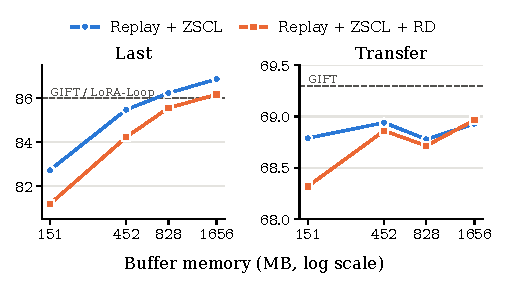
\includegraphics[width=\linewidth]{figs/q2a_budget.pdf}
  \caption{\textbf{\Q{2}: performance vs.\ replay budget} (log-scale MB). \TODO{Last and Transfer, with and without $\Lrd$.}}
  \label{fig:q2a}
\end{figure}

\subsection{Selection (\Q{2}, \Q{3})}
\label{sec:res-select}
\TODO{Summary only: does any strategy beat random, and at which budget? One sentence for images (\Q{2}), one for features (\Q{3}). Full tables in \cref{sec:abl-select}.}

\subsection{Quantization (\Q{3})}
\label{sec:res-quant}
\TODO{Gist: how far precision can drop before accuracy falls; headline point on the PQ curve. Full sweep in \cref{sec:abl-quant}.}

%%%%%%%%%%%%%%%%%%%%%%%%%%%%%%%%%%%%%%%%%%%%%%%%%%%%%%%%%%%%%%%%%%%%%%%%%
\section{Ablations}
\label{sec:ablations}

\subsection{Budget and distillation (\Q{2})}
\label{sec:abl-budget}
\TODO{Budget sweep with and without $\Lrd$ (\cref{tab:q2a}). Does distillation matter more when the buffer is small?}

\begin{table}[t]
\centering
\small
\setlength{\tabcolsep}{3.5pt}
\caption{\textbf{\Q{2}: replay budget.} Image replay with $\Lzscl$, with
and without $\Lrd$ ($\lambda{=}0.3$, per-task iteration schedule). Memory
assumes uint8 images (150.5\,kB each). Single seed.}
\label{tab:q2a}
\begin{tabular}{@{}rrr cc cc@{}}
\toprule
& & & \multicolumn{2}{c}{Replay + ZSCL} & \multicolumn{2}{c}{+ RD} \\
\cmidrule(lr){4-5}\cmidrule(lr){6-7}
Samples & /class & MB & Transfer & Last & Transfer & Last \\
\midrule
1k     & 0.8 & 151  & 68.79 & 82.73 & 68.32 & 81.18 \\
3k     & 2.4 & 452  & 68.94 & 85.48 & 68.86 & 84.23 \\
5.5k   & 4.4 & 828  & 68.78 & 86.23 & 68.71 & 85.56 \\
11k    & 8.8 & 1656 & \tbd  & \tbd  & 68.96 & 86.17 \\
44k    & \tbd & \tbd & \tbd & \tbd & \tbd & \tbd \\
All    & \tbd & \tbd & \tbd & \tbd & \tbd & \tbd \\
\bottomrule
\end{tabular}
\end{table}

\subsection{Selection strategies (\Q{2}, \Q{3})}
\label{sec:abl-select}
\TODO{Detailed comparison at a scarce and a saturated budget, for images (\cref{tab:q2b}) and features (\cref{tab:q3c}).}

\begin{table}[t]
\centering
\small
\setlength{\tabcolsep}{3.5pt}
\caption{\textbf{\Q{2}: selecting images.} Evaluated where the buffer is
scarce (1k) and where it is saturated (11k). Top: how the budget is split
($^\ddagger$1500 it./task, no $\Lrd$). Bottom: which samples are kept within a
class (full method, per-class allocation). Single seed.}
\label{tab:q2b}
\begin{tabular}{@{}ll cc cc@{}}
\toprule
& & \multicolumn{2}{c}{1k samples} & \multicolumn{2}{c}{11k samples} \\
\cmidrule(lr){3-4}\cmidrule(lr){5-6}
Strategy & Criterion & Transfer & Last & Transfer & Last \\
\midrule
Equal per task$^\ddagger$  & allocation & \tbd & \tbd & 69.02 & 86.44 \\
Equal per class$^\ddagger$ & allocation & \tbd & \tbd & 69.03 & 86.44 \\
\midrule
Random            & --                 & 68.32 & 81.18 & \best{68.96} & \best{86.17} \\
Herding           & class-mean match   & \tbd & \tbd & 68.42 & 86.11 \\
Surprisal (EL2N)  & high error         & \tbd & \tbd & 68.56 & 85.97 \\
GCR               & gradient coreset   & \tbd & \tbd & 68.27 & \best{86.17} \\
Coverage          & $k$-center         & \tbd & \tbd & 68.73 & 86.12 \\
\bottomrule
\end{tabular}
\end{table}

\begin{table}[t]
\centering
\small
\setlength{\tabcolsep}{3.5pt}
\caption{\textbf{\Q{3}: selecting features.} The \Q{2} strategies applied
in embedding space.}
\label{tab:q3c}
\begin{tabular}{@{}l cc cc@{}}
\toprule
& \multicolumn{2}{c}{1k features} & \multicolumn{2}{c}{11k features} \\
\cmidrule(lr){2-3}\cmidrule(lr){4-5}
Strategy & Transfer & Last & Transfer & Last \\
\midrule
Random            & \tbd & \tbd & 68.60 & 84.79 \\
Herding           & \tbd & \tbd & \tbd & \tbd \\
Surprisal (EL2N)  & \tbd & \tbd & \tbd & \tbd \\
Coverage          & \tbd & \tbd & \tbd & \tbd \\
\bottomrule
\end{tabular}
\end{table}

\subsection{Quantization (\Q{3})}
\label{sec:abl-quant}
\TODO{Full sweep (\cref{tab:q3d}): embedding precision and PQ bit rate. Accuracy vs.\ reconstruction error.}

\begin{table}[t]
\centering
\small
\setlength{\tabcolsep}{3.5pt}
\caption{\textbf{\Q{3}: quantization.} Top: precision of the final embedding.
Bottom: product quantization of mid-network tokens; $m$ = sub-quantizers,
error floor $= 2^{-R}$. Memory at $N{=}$11k.}
\label{tab:q3d}
\begin{tabular}{@{}l rr c cc@{}}
\toprule
Format & Bytes/sample & MB & Error & Transfer & Last \\
\midrule
\multicolumn{6}{@{}l}{\emph{Final embedding (512-d)}} \\
fp32           & 2048    & 22.5 & 0    & \tbd  & \tbd \\
fp16           & 1024    & 11.3 & \tbd & 68.60 & 84.79 \\
int8           & 512     & 5.6  & \tbd & \tbd  & \tbd \\
int4           & 256     & 2.8  & \tbd & \tbd  & \tbd \\
\midrule
\multicolumn{6}{@{}l}{\emph{Mid-network tokens (PQ, tap block 6)}} \\
fp16 (no PQ)   & \tbd    & \tbd & 0     & \tbd  & \tbd \\
$m{=}128$      & 25.2\,k & 277  & 0.397 & 68.91 & \best{85.88} \\
$m{=}64$       & 12.6\,k & 139  & 0.630 & 68.83 & 84.72 \\
$m{=}32$       & 6.3\,k  & 69   & 0.794 & 68.73 & 83.66 \\
\bottomrule
\end{tabular}
\end{table}

%%%%%%%%%%%%%%%%%%%%%%%%%%%%%%%%%%%%%%%%%%%%%%%%%%%%%%%%%%%%%%%%%%%%%%%%%
\section{Discussion}
\label{sec:discussion}

\subsection{What replay adds to distillation (\Q{1})}
\label{sec:disc-q1}
\TODO{Interpretation of \cref{tab:q1}: which component carries which metric; whether forgetting or plasticity is the binding constraint.}

\subsection{Storing features instead of images (\Q{3})}
\label{sec:disc-q3a}
\TODO{Memory saved vs.\ accuracy cost at the same $N$ (\cref{tab:q3ab}). Where the cost comes from: stale features, damage grows with task age (\cref{tab:drift}). Whether drift correction helps.}

\begin{table}[t]
\centering
\small
\setlength{\tabcolsep}{4pt}
\caption{\textbf{\Q{3}: feature drift.} Per-task Last for the oldest tasks,
and the effect of drift correction on stored embeddings.}
\label{tab:drift}
\begin{tabular}{@{}l ccc c@{}}
\toprule
Buffer & Aircraft & CIFAR100 & DTD & Last (all) \\
\midrule
Images                       & 54.52 & 81.98 & 76.06 & 86.17 \\
Embedding, no correction     & 44.55 & 79.74 & 74.73 & 84.79 \\
\quad + SDC (image anchors)  & 46.74 & 78.26 & 74.52 & 84.65 \\
\quad + LP (text anchors)    & 44.85 & 79.77 & 74.89 & 84.73 \\
\quad + LP (both)            & 46.23 & 79.06 & 75.80 & 84.89 \\
\bottomrule
\end{tabular}
\end{table}

\subsection{Memory-matched features (\Q{3})}
\label{sec:disc-q3b}
\TODO{Fill the image buffer's bytes with features (\cref{tab:q3ab}, \cref{fig:pareto}). Does quantity make up for staleness? Where the storage forms cross over.}

\begin{table*}[t]
\centering
\small
\caption{\textbf{\Q{3}: what to store.} \emph{Same $N$} keeps the
sample count of image replay (\Q{3}). \emph{Same MB} fills the image buffer's
memory with features (\Q{3}). Embedding: final 512-d image feature.
Tokens: product-quantized mid-network tokens.}
\label{tab:q3ab}
\begin{tabular}{@{}ll rrr ccc@{}}
\toprule
Stored form & Setting & Bytes/sample & \# Samples & Memory (MB)
            & Transfer & Avg. & Last \\
\midrule
Images (uint8)       & reference & 150\,kB & 11k  & 1656 & 68.96 & 77.17 & 86.17 \\
\midrule
\multirow{2}{*}{Embedding (fp16)}
                     & same $N$  & 1\,kB   & 11k  & 11   & 68.60 & 76.08 & 84.79 \\
                     & same MB   & 1\,kB   & \tbd & \tbd & \tbd & \tbd & \tbd \\
\midrule
\multirow{2}{*}{Tokens (PQ, $m{=}128$)}
                     & same $N$  & 25\,kB  & 11k  & 277  & 68.95 & 76.86 & 86.04 \\
                     & same MB   & 25\,kB  & \tbd & \tbd & \tbd & \tbd & \tbd \\
\bottomrule
\end{tabular}
\end{table*}

\begin{figure}[t]
  \centering
  \fbox{\rule{0pt}{1.2in}\rule{0.9\linewidth}{0pt}}
  %\includegraphics[width=\linewidth]{figs/pareto_memory.pdf}
  \caption{\textbf{\Q{3}: Last vs.\ buffer memory} for all storage forms (log-scale MB). \TODO{Mark the Pareto frontier.}}
  \label{fig:pareto}
\end{figure}

\subsection{Quantity vs.\ fidelity (\Q{3})}
\label{sec:disc-q3d}
\TODO{At fixed bytes, is it better to store more low-precision samples or fewer exact ones?}

\subsection{Answers and recommendations}
\label{sec:answers}
\TODO{One short paragraph per question, answering it directly.}
\textbf{\Q{1}:} \TODO{}
\textbf{\Q{2}:} \TODO{}
\textbf{\Q{3}:} \TODO{}

\paragraph{Limitations.}
\TODO{Single benchmark, backbone, task order; number of seeds.}

\paragraph{Future directions.}
\TODO{\Q{3} follow-ups: feature-level augmentation, refreshing stored features, a previous-task teacher for feature distillation, other backbones.}

%%%%%%%%%%%%%%%%%%%%%%%%%%%%%%%%%%%%%%%%%%%%%%%%%%%%%%%%%%%%%%%%%%%%%%%%%
\section{Conclusion}
\label{sec:conclusion}

\TODO{Conclusion.}

%%%%%%%%%%%%%%%%%%%%%%%%%%%%%%%%%%%%%%%%%%%%%%%%%%%%%%%%%%%%%%%%%%%%%%%%%
{
    \small
    \bibliographystyle{ieeenat_fullname}
    \bibliography{cvpr-2027/papers}
}

\end{document}
